\subsubsection{Efficiency Improvement}
\label{subsubsec:overall-sw}

\begin{figure}[h]
\vspace{-8pt}
	\centering
		\subfloat[Average $rEFF_{SW}$] {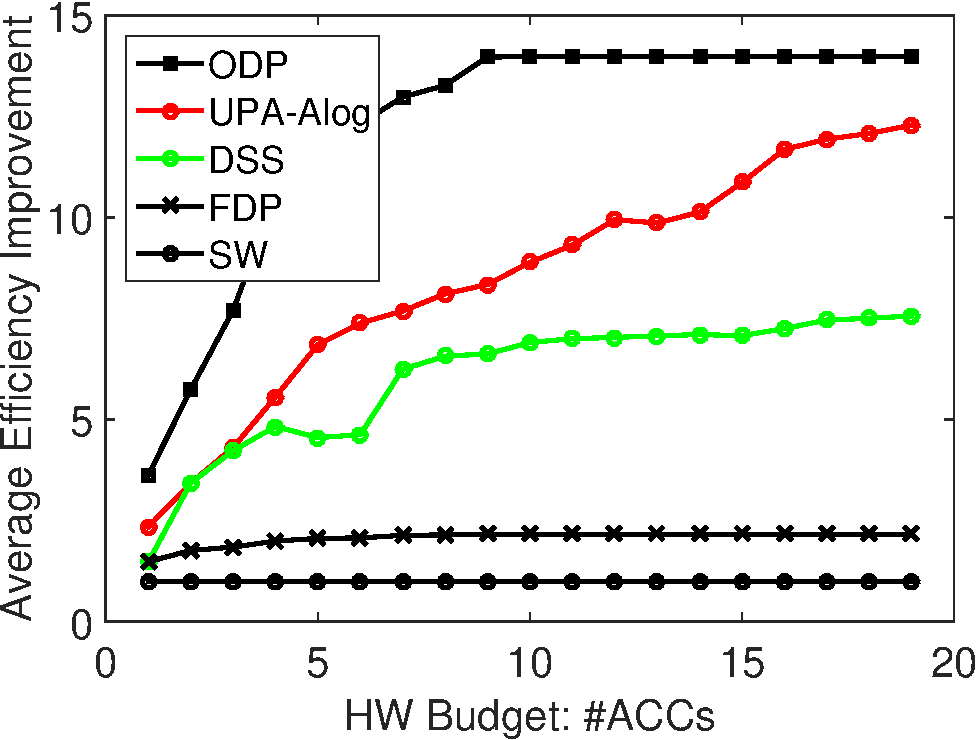
\includegraphics[width=.48\linewidth]{fig/allsw.pdf}\label{fig:allsw}}
		\hfill
		\subfloat[Cumulative Probability (ACCs=12)] {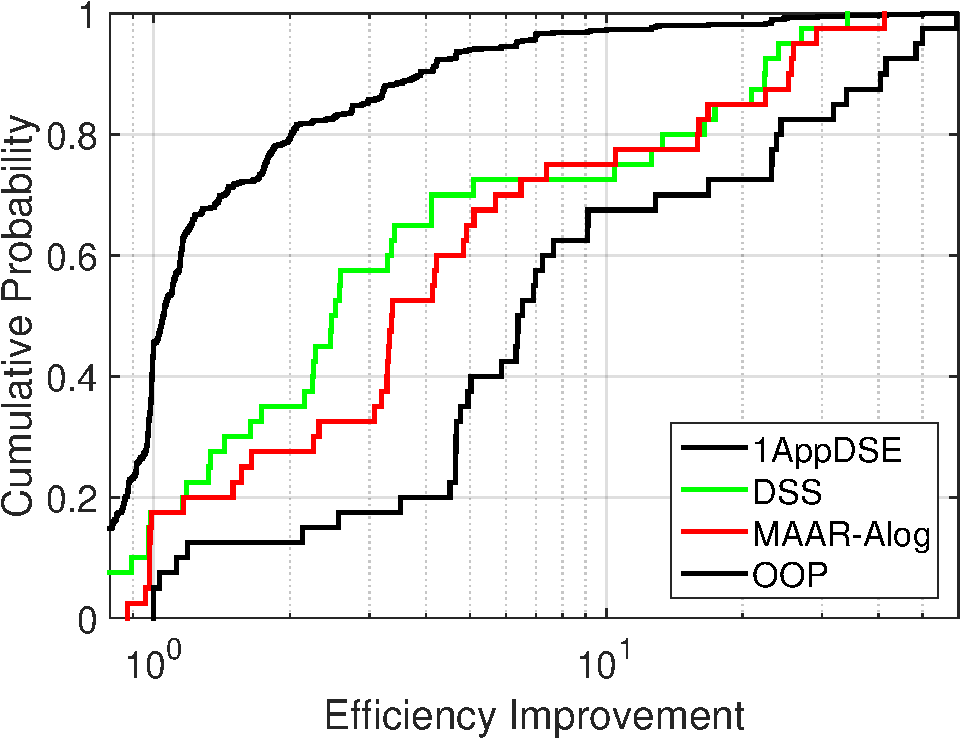
\includegraphics[width=.48\linewidth]{fig/MAARsw12all.pdf}\label{fig:sw12all}}
	\vspace{-8pt}
	\caption{Efficiency Improvement $rEFF_{SW}$}
	\label{fig:overallsw}
\end{figure}

\newtext{
\figref{fig:allsw} shows the average efficiency improvement ($rEEF_{SW}$) across all applications of different platform allocations over increasing ACCs budgets. ODP yields the absolute upper bound for a given HW constraints. ODP plateaus after ACCs=9, since each application only has up to 10 unique kernels. Since SW compared with itself, the $rEFF_{SW}$ value of SW is always equal to 1, which yields the lower bound. UPA uses $Alog$ (log area aggregation of $EEF$) evaluation. UPA-Alog's average efficiency improvement increases with the number of ACCs. It approaches the ODP efficiency when ACCs=19. With a 12 ACCs budget, UPA-Alog has 1.41 times the average efficiency improvement of DSS, and 4.59 times the improvement of FDP.
}

\newtext{
To give a detail comparison among different allocations, 
\figref{fig:sw12all} shows the cumulative probability of efficiency improvement for ODP, UPA, DSS and FDP with a ACCs=12 budget.} 
The x-axis denotes efficiency improvement ($rEFF_{SW}$), and y-axis is the cumulative probability.
A point ($x$, $y$) indicates that a proportion $y$ of applications have a relative efficiency $x$ or less.  
E.g. there is 67.5\% (0.675 in y-axis) probability that ODP has 10x ($10^1$ in x-axis) or 10x less efficiency improvement. In another description, ODP has 32.5\% ($1-0.675$ in y-axis) to achieve 10x or 10x more efficiency improvement. 

In \figref{fig:sw12all}, the line positioned more toward the bottom right has a better efficiency improvement, and ODP black line is the upper bound. 
\newtext{
SW can be considered as the lower bound, which has constant 1 efficiency improvement (i.e. vertical line $x = 10^0$ if drawn). 
As \figref{fig:sw12all} shown, UPA-Alog (red line) improves efficiency more than FDP (up left black line) and DSS (green line) for almost all applications. 
67.5\% ($1-0.325$ in y-axis) of applications have at least a 3x improvements, while FDP and DSS only improve 15\% ($1-0.85$) and 42.5\% ($1-0.575$) of applications respectively by the same amount. 
Note that FDP has a more smooth line, and shows more detail as it considers running any application on any application's dedicated optimal platform. 
}